\section{Morbillo}

Importanza del problema oggi:

\begin{itemize}
\item
  È ancora presente come malattia
\item
  È ancora una causa importante di morte per i bambini, prevalentemente
  nei paesi in via di sviluppo, nonostante la disponibilità di un
  vaccino dagli anni `60
\item
  Le campagne di vaccinazione che sono state portate avanti almeno dagli
  anni 2000, hanno ottenuto una riduzione delle morti (dati del 2008)
  del 70\%. Nel 2014 sono stati segnalati ancora circa 120000 morti e di
  questi il 95\% è nei paesi con condizioni igienico-sanitarie non
  ottimali.
\end{itemize}

\subsection{Caratteristiche e Cenni clinici}

Il morbillo è una malattia ad eziologia virale, altamente contagiosa,
specie specifica (colpisce solo l'uomo), tipicamente endemio-epidemica.

In epoca prevaccinale era la classica malattia dell'infanzia. È molto
diffusa in tutto il mondo e molto grave nei paesi in via di sviluppo.

L'agente eziologico è un virus ad RNA (Paramyxovirus), dotato di un
pericapside con un antigene di superficie, che protrude dal peplus, e
che rappresenta il recettore del virus per le cellule sensibili e che è
anche l'antigene immunogeno protettivo.

È noto un solo tipo di antigene anche se oggi con le moderne tecnologie
sono identificati numerosi genotipi.

È un virus molto fragile, facilmente aggredibile da agenti esterni
(calore, luce, disinfettanti).

È un virus a trasmissione aerea. Penetra per via aerea e si replica
nelle cellule naso-faringee e nei linfonodi regionali; parte la prima
viremia dopo 2-3 giorni dall'esposizione, seguita successivamente da una
seconda fase viremica, nella quale il virus diffonde a livello cutaneo (
fase esantematica ).


\subsection{Andamento della malattia}

Ha un periodo lunghissimo di incubazione, circa 1-2 settimane.

Fase prodromica con febbre elevata,
macchie di Koplik, tosse, rinite, congiuntivite.

Compare quindi il rash cutaneo che dura 5-6 giorni, ha una diffusione
cranio-caudale con scomparsa nello stesso ordine di giorni.

Ha una prognosi benigna nel bambino sano, ma può presentare delle
complicanze:

\begin{itemize}
\item
  Di tipo respiratorio età-specifiche (nel bambino \textless{} 5 anni) e
  sono: trachebronchiti, broncopolmoniti, polmoniti da virus (1-7\%) e
  otite media (7-9\%)
\item
  Di tipo neurologico che si presentano tipicamente nella seconda
  infanzia (dopo i 9 anni):

\begin{itemize}
\item
  Encefalite post morbillosa, abbastanza rara con incidenza di 1-2 casi
  ogni 1000 malati 
\item
  Panencefalite sclerosante subacuta (SSPE) con letalità totale (100\%)
  ma molto rara 0,5-3 casi/milione/anno nel mondo. Si tratta di una
  forma degenerativa del SNC (patologia demielinizzante), correlata ad
  un'infezione da morbillo acquisita precocemente (nel primo anno di
  vita o addirittura quando è lattante). La causa è la persistenza del
  virus modificato a livello dell'encefalo. Tramite studi degli
  anticorpi nel liquor è stata dimostrata l'assenza di una componente
  anticorpale verso una delle proteine del virus (proteina M), che gioca
  un ruolo importante nella replicazione rendendolo più lento e quindi
  consentendogli questa resistenza. I primi segni (cambio di
  personalità, degenerazione cognitiva) si osservano a distanza di 8
  anni dalla malattia morbillosa (età del soggetto: 8-10 anni). La
  sopravvivenza è molto modesta, 1-2 anni. 
\end{itemize}
\end{itemize}

\subsection{Epidemiologia e Profilassi}

Nel morbillo possiamo considerare tre fasi:

\begin{itemize}

\item[1.]
 EPOCA
  PREVACCINALE: prima degli anni '60 quando non c'era un vaccino,
  caratterizzata da andamento epidemico ogni 2-3 anni: la nuova ondata
  di nuovi nati forniva il materiale perché il virus potesse esprimersi.
\item [2.]
  VACCINAZIONE AL FINE DI CONTROLLARE LA MALATTIA MORBILLOSA: a partire
  dagli anni '60-'70. Caratterizzata da incidenza minore, focolai
  epidemici contenuti, ma vi è tendenza a esprimersi nella seconda
  infanzia e nel giovane adulto.
\item[3.]
  VACCINAZIONE AL FINE DI ERADICARE LA MALATTIA: a partire dal 2000
\end{itemize}

\begin{figure}[!ht]
\centering
	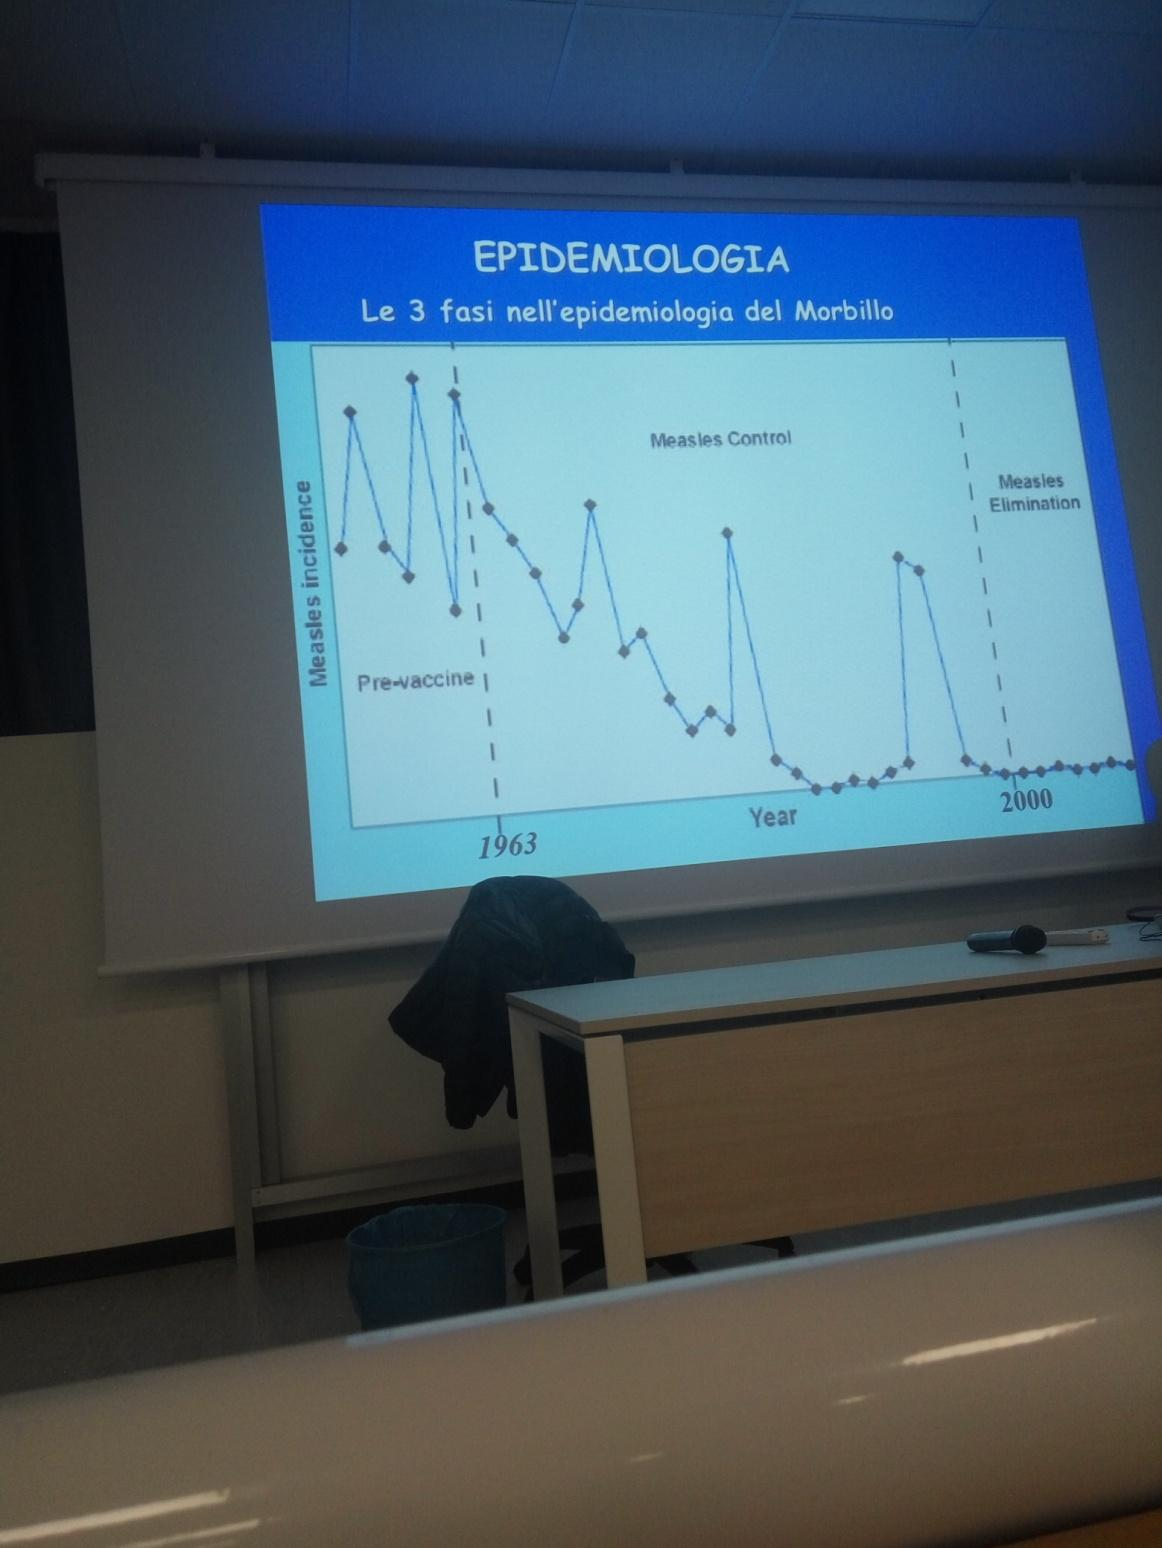
\includegraphics[width=0.8\textwidth]{07/image1.jpeg}
	\end{figure}

Nei PAESI SOTTOSVILUPPATI: a causa di famiglie molto numerose, ambienti
affollati, condizioni igieniche precarie, condizioni di malnutrizione,
la patologia ha ancora una grande diffusione, con frequenti complicanza
e elevata letalità.

Nei PAESI INDUSTRIALIZZATI la situazione è diversa: le campagne di
vaccinazione estese hanno portato certamente ad una riduzione della
patologia, ma non ad un'eradicazione. Quindi di fatto si ha uno
spostamento della malattia verso un'età più avanzata, non più un
problema della prima infanzia ma problema possibile per la seconda
infanzia o per l'adulto\emph{.} È un fenomeno paradosso perché, se il
bambino non ha la possibilità di contrarre il virus nell'epoca classica
dell'infanzia, è possibile che lo incontri in adolescenza o anche in età
adulta, dove la malattia è molto più pericolosa.

In ITALIA si partiva negli anni '90 con oltre 30000 casi, poi ci sono
state due grandi epidemie recenti come quella del 2002 (circa 18000
casi) per infine ridursi a circa 200-300 casi/anno.

Nel 2007 ci fu un focolaio in Piemonte, causato da una ragazza di 17
anni al ritorno di una vacanza studio in Inghilterra; ha infettato
compagni e amici che come lei erano suscettibili.

Nel 2013-2014 c'è stato un ritorno del morbillo in tutta l'Europa
causata da casi di importazione.

Una malattia infettiva finché non avviene l'eradicazione è un problema
anche dove da molto tempo non si verifica più un caso se esistono dei
suscettibili.

\subsection{Sorgente d'infezione}

È un virus esclusivamente umano quindi la sorgente d'infezione è l'uomo.
Il periodo di contagiosità va dai 4-5 giorni prima della comparsa del
rash, fino a 4-5 giorni dopo.

Il lungo periodo di incubazione permette eliminazione del virus ben
prima che esprima una condizione di malattia. Perciò se il bambino
incontra individui suscettibili può essere causa di una piccola
epidemia. Non esistono portatori sani.

La trasmissione è aerea con contatto stretto con il malato o con
trasmissione semindiretta. La forza del virus è di poter resistere nei
nuclei essiccati delle goccioline di flugge nell'aria.

La stagionalità, come per tutte le malattie dell'albero respiratorio, è
legata alla fine dell'inverno e inizio primavera.

\subsection{Prevenzione}

\begin{itemize}
\item
  \emph{Denuncia Obbligatoria} {[}Classe II{]}
\item
  Accertamento Diagnostico (poco importante, anche perché dal punto di
  vista clinico è molto caratteristica
\item
  Isolamento: è importante per motivi terapeutici nel caso si tratti di
  situazioni critiche, per la tutela del paziente. È in genere un
  isolamento in casa per separare il malato dalla comunità.
\item
  \emph{Disinfezione Continua} associata a ventilazione degli ambienti
\item
  \emph{Profilassi Immunitaria Specifica:} caratterizzante la
  prevenzione, che comprende Vaccino Profilassi (Attiva) e Siero
  Profilassi (Passiva).
\end{itemize}

\subsection{Immunoprofilassi Attiva}

La sua storia parte da lontano; virus
isolato negli anni: nel 1968 I vaccino vivo attenuato
(Edmonson-Enders-Strain), nel 1971 Diventa un vaccino associato, con 3
componenti Ag importanti, Morbillo Rosolia Parotite (MRP trivalente) e
nel 1989 Modifica della scheda vaccinale da 1 singola dose a 2 dosi
volte alla eradicazione (che si può ottenere con la copertura vaccinale
di oltre il 92\% della popolazione mondiale).

Efficacia e elevatissima, sovrapponibile quella del monovalente con
quella del trivalente.

Efficacia 95\% (Range 90-98\%)

Durata : Duratura, si ritiene duri tutta la vita (come avviene nelle
infezioni naturali) Schedula 1 + 1 (la vaccinazione di base richiede 1
sola dose/somministrazione, la seconda è stata aggiunta per motivi
epidemiologici e di strategia vaccinale).

Negli ultimi anni si è resa disponibile anche la vaccinazione
tetravalente (comprende anche la Varicella).

Come si vorrebbe ottenere l'eradicazione a livello mondiale secondo
l'OMS - PNEMORC = piano nazionale per l'eliminazione di morbillo e
rosolia congenita.

\begin{itemize}
\item
Aumentando la sorveglianza epidemiologica.
\item
  Vaccinazioni supplementari nei paesi sottosviluppati che spesso e
  laddove e più grave per
\item
  diffusione e letalità.
\item
  Migliorando il trattamento dei casi di malattia, nel III mondo e una
  gravissima malattia dell'infanzia
\item
  è tra le prime cause di morte infantile.
\item
  Migliorando le campagne vaccinali, difficile per i vaccini vivi, serve
  coordinazione e non è sempre facile portare il vaccino dove serve
  senza che questo si denaturi
\item
  co-somministrazione di vitamina A che migliora lo stimolo antigenico
  (malnutrizione peggiora la gravità della malattia).
\end{itemize}

\subsection{Indicazioni alla vaccinazione}

\begin{itemize}
\item[1.]
  Tutti i bambini tra il 12\textsuperscript{o} e il 15\textsuperscript{o} mese (Gli Ab materni che passano
  all'atto della nascita al neonato sono i più duraturi come immunità
  passiva naturale e quindi neutralizzerebbero il vaccino se questo
  venisse fatto prima del tempo stabilito) 
\item
  Adulti e adolescenti suscettibili
\end{itemize}

\subsection{La strategia vaccinale in Italia}

Si ottiene con:

\begin{itemize}
\item
  Vaccinazione di MASSA di tutti i nuovi nati tra 12\textsuperscript{o} e 15\textsuperscript{o} mese.
\item
  Ulteriore dose vaccinale tra 6\textsuperscript{o} e 12\textsuperscript{o} anno. E' una fascia larga. Ogni
  USL decide esattamente in quale momento di questo intervallo attuare
  la vaccinazione sul suo territorio; questa seconda dose serve per:
\begin{itemize}
\item
  Indurre immunità nei non responders (in cui ha fallito la I dose, sono
  2-5\%) a causa di: 

  \begin{itemize}
  \item
    Cattiva conservazione del vaccino
  \item
    Soggetto è di per sé non responder (in genere alla seconda
    somministrazione rispondono)
  \end{itemize}
\item
  Quelli non vaccinati al I step, perché non è obbligatoria, vengono qui
  ``catturati''
\end{itemize}
\end{itemize}

Il vaccino è da sempre su base volontaria, non sono stati ottenuti i
risultati sperati; vi erano zone ed USL che lavoravano bene e altre che
lavoravano un po' meno bene, creando sul territorio nazionale una
situazione a ``macchia di leopardo'' tale da non poter garantire
l'interruzione della circolazione del virus e addirittura creando un
effetto paradosso, ovvero far si che l'incontro con il virus avvenisse
più tardi nella vita del soggetto, quando cioè le manifestazioni
cliniche sono più gravi (II, III infanzia). Nel 2000 ci si è allineati
con l'intento dell'OMS di eradicare la malattia, attraverso una spinta
molto forte verso la vaccinazione. Rimane volontaria ma è intensificato
l'invito ad eseguirla.

Negli adulti il vaccino è lo stesso, consigliato nei soggetti a rischio,
per la vita di comunità:

\begin{itemize}
\item
  Studenti di College
\item
  Viaggiatori internazionali
\item
  Personale sanitario
\item
  Personale scolastico
\end{itemize}

L'immunità antimorbillosa è accertabile tramite:

\begin{itemize}
\item
  Il dato anamnestico che è sovrapponibile al dato sierologico per il
  morbillo; quando la madre o il medico dicono che l' ha avuto, allora
  l' ha avuto per davvero.
\item
  Si può verificare comunque anche sierologicamente.
\item
  tener buona nel 99\% dei casi la scheda vaccinale.
\end{itemize}

\subsection{Effetti Collaterali}

\begin{itemize}
\item
  Febbre modica 5-10\%
\item
  Rash 5\%
\item
  Atralgie 25\%
\item
  Trombocitopenia
\item
  Parotite
\item
  Difetti dell'udito (legati a ceppo parotitico)
\item
  Encefalopatia rara
\end{itemize}

\subsection{Precauzioni e Controindicazioni}

\begin{itemize}
\item
  Immunodepressione (è un vaccino vivo)
\item
  Gravidanza
\item
Reazioni allergiche preesistenti a
  componenti del vaccino o sviluppate dopo I somministrazione (dovute
  alla preparazione da uovo o embrione, perché morbillo e parotite si
  coltivano nelle uova embrionali di pollo). In alcuni preparati possono
  esserci tracce di antibiotici (penicillina), per le piastre di
  coltivazione, quindi soggetti allergici a queste molecole, possono
  avere reazioni.
\item
  Malattia acuta in atto
\item
  Somministrazione recente di IgG (possono bloccare il vaccino e
  viceversa)
\end{itemize}

Molti dei vaccini, al momento dell'immissione sul mercato hanno avuto
dei contrasti, infatti in alcuni casi sono stati ritirati dal mercato.
Uno dei principali problemi per il vaccino del morbillo è l'associazione
con alcune patologie, in particolare con l' \textbf{Autismo.}

Pubblicazione sul ``Lancet'' da parte di un gastroenterologo inglese
negli anni '90. Associava lo sviluppo di Autismo alla vaccinazione
contro il Morbillo. Sono partiti molti studi a riguardo, sponsorizzati
dall'OMS. Hanno dimostrato di come \textbf{non} sussista tale
correlazione. Nel 2008 esce la fase finale con studi caso controllo in
cui si dimostra la non associazione. Nel 2010 la sentenza di tribunale
che sanciva che l'autore e la rivista avessero pubblicato un articolo
scientificamente non affidabile.

\subsection{Immunoprofilassi Passiva}

Ig: Indicazione ( A seconda della tempistica di somministrazione)

Normali

Specifiche

Non c'e differenza di efficacia tra Normali e Specifiche.

Nelle Normali la quota di Ab è
consistente, può essere usato per la protezione eccezionale: si usano
come misura di emergenza nel caso che il contagio si sia già realizzato
o è molto probabile e bisognerebbe darle entro 96 ore dal contatto.

A volte si sceglie di attenuare la malattia, non impedendo l'infezione o
la malattia stessa, di modo da far immunizzare il paziente con una
malattia più blanda che aumenta comunque il suo titolo di Ab.

Si possono fare in quei casi in cui il rischio di avere una forma grave
è elevato a causa di condizioni predisponenti, come, ad esempio, nel
lattante che ha un fratello che va a scuola . Si decide, quindi, di
difendere il lattante preventivamente con le immunoglobuline. È una
protezione limitata nel tempo (4-5 settimane) dopo il soggetto torna ad
essere nelle stesse condizioni di partenza.


\section{Rosolia}
Malattia infettivo contagiosa nella quale riconosciamo due destinatari:
uno è l'adulto e l'altro è il prodotto del concepimento o il neonato.

Forma Post-Natale: benigna, ma bimodale perché colpisce sia bambini
piccoli che giovani adulti.

Forma connatale: prima infezione contratta in gravidanza da una donna
suscettibile.

\subsection{Caratteristiche del patogeno}

Il
virus fa parte della famiglia Togaviridae, genere Rubivirus, è un virus
di medie dimensioni dotato di pericapside; è presente un solo tipo
antigenico; il pericapside rende il virus particolarmente fragile e
passibile di distruzione ad opera di agenti fisici e chimici quali i
raggi UV, basso pH, solventi, calore.

La trasmissione avviene tipicamente per via aerea, il virus replica a
livello del nasofaringe e nei linfonodi regionali, entra in circolo
dando luogo ad una viremia persistente, che inizia 5-7 giorni dopo
l'esposizione, ovvero prima della manifestazione della malattia,
successivamente il virus diffonde agli organi e ai tessuti. Durante il
periodo di viremia, le particelle virali possono attraversare la
placenta e infettare il feto.

Incubazione di 14-23 giorni.

Può essere paucisintomatica e non
essere riconosciuta. I segni più evidenti sono la comparsa di una
linfadenopatia, rash fugace (simile al morbillo) e nel 50\% dei casi è
asintomatica.

Le complicanze principali sono: artralgia (donne adulte 25\%) e molto
rare l'encefalite, trombocitopenia, porpora, neurite e orchite.

\subsection{Storia naturale dell'infezione}

È presente un lungo periodo d'incubazione, così che al momento
dell'eventuale comparsa di sintomi abbiamo già un periodo viremico alle
spalle rilevante, che dura comunque ancora 5-7 giorni. Ancora più lungo
è il periodo d'eliminazione dall'orofaringe. La concentrazione del virus
è massima nel periodo che va da 5 giorni prima a 7 giorni dopo
l'esordio.

L'immunità è duratura. La madre conferisce un'immunità passiva al
neonato per una durata di circa 4-6 mesi, tramite IgG, capaci di passare
la barriera placentare.

Quando la prima infezione avviene \textbf{in corso di gravidanza} in una
donna non immune il feto è esposto al virus: le conseguenze possono
essere molto serie e vanno dal danno fetale all'aborto; mentre quando la
rosolia è contratta all'atto della nascita si manifesta con cataratta
congenita, segno classico di infezione da rosolia in corso di
gravidanza.

Non è sempre detto che virus passi la placenta e in questo caso neonato
è sano.

Il danno è causato dal fatto che il virus penetra per via placentare,
replica, provoca necrosi dei vasi sanguigni, le cellule infettate
arrivano al feto che va incontro a infezione: si verifica interferenza
con la mitosi. Le cellule possedute dal neonato alla nascita risultano
in numero minore del normale. Quanto più è precoce l'infezione, tanto
più amplificato è il danno:

\begin{itemize}
\item
  1\textsuperscript{o} mese: danni attribuibili all'infezione = 50-70\% , + 8\% relativo
  agli aborti
\item
  2\textsuperscript{o} mese: 30\% dei danni
\item
  3\textsuperscript{o} mese: 8-15\%,
\item
  4\textsuperscript{o} mese: 0,1-3\%. (trascurabile)
\end{itemize}

Il bambino può inoltre essere sano alla nascita ma sviluppare
complicanze tardive.

\subsection{Principali malformazioni e danni} 

\begin{itemize}
\item
  Affezioni oculari 71\%
\item
  Sordità 69\%: difetti a carico del nervo
\item
  Malformazioni cardiache 49\%: difetti settali, pervietà del dotto di
  Botallo
\item
  SNC 45\%: ritardo psicomotorio, microcefalia, encefalite
\end{itemize}

Raramente si ha la presentazione di una singola malformazione,
ricordiamo la correlazione del danno col primo mese di gestazione e
progressivamente la caduta del danno.

\subsection{Criteri per correlare alla rosolia un'infezione congenita o una sindrome congenita}

\begin{itemize}
\item
  Aborto spontaneo
\item
  Difetti cardiaci molteplici (pervietà del dotto di Botallo,difetti
  interatriali e interventricolari, a carico dei grossi vasi)
\item
  SNC (ritardo mentale, microcefalia,encefalite)
\item
  Sordità (correlata al danno al SNC)
\item
  Endocrinopatie
\item
  Difetti dell'occhio (cataratta, glaucoma, macroftalmia, retinopatie)
\item
  Alterazioni dell'apparato genito-urinario
\item
  Alterazioni di carattere ematologico (anemia, trombocitopenia)
\item
  Epatiti (si esprimono più tardi)
\item
  Disordini psichiatrici
\end{itemize}

\subsection{Accertamento diagnostico}

Materiali di scelta sono il tampone
faringeo e le urine.

Il tampone faringeo permette sia accertamento diretto con ricerca del
virus, che accertamento indiretto con la ricerca degli anticorpi (2
campioni per IgG, uno solo per IgM).

Accertamento Diagnostico è importante per verificare se le donne in età
fertile sono suscettibili o protette (Rubeotest - ricerca IgG
specifiche).

\subsection{Epidemiologia}

Si tratta di un'infezione presente in tutto il mondo, ampia è la quota
di soggetti infetti non malati; l'andamento è endemo-epidemico, con
epidemie cicliche ogni 6-9 anni, soprattutto tra la fine dell'inverno e
la primavera (tipica fragilità della mucosa, maggior probabilità di
attecchimento del virus, condivisione da parte dei soggetti di spazi
chiusi e talvolta poco aerati).

L'età di comparsa vede due picchi: tra i 5 e i 15 anni e nel giovane
adulto (> 20 anni).

\subsection{Serbatoi di infezione}

È un virus specie-specifico, pertanto
l'uomo è l'unico serbatoio d'infezione.

\begin{itemize}
\item
  malato: infettante e contagiante da circa 5-7 giorni prima a circa 5-7
  giorni dopo l'esantema
\item
  portatore precoce
\item
  portatore asintomatico
\item
  neonato infetto: eliminazione virale abbondantissima e lunghissima,
  ravvisabile anche 18 mesi dopo la nascita, con potenziale acquisizione
  da parte degli altri bambini e di chi li accudisce
\end{itemize}

\subsection{Modalità di trasmissione}

\begin{itemize}
\item
diretta per rapporti affettuosi
  madre-bambino o fra adulti
\item
  semidiretta attraverso liquidi biologici quali le urine
\end{itemize}

Nonostante la vaccinazione sia molto sentita, ci sono ancora molti
suscettibili (almeno 5\% di donne suscettibili in età fertile). La
riduzione dei casi è partita dagli anni '90 con l'introduzione del
vaccino.

Dal 2000 le Americhe sono state giudicate Rosolia free (non ci sono più
casi autoctoni), ci sono casi seppur non numerosi dovuti all'ingresso di
persone infette.

\subsection{Profilassi}

In Italia è una patologia soggetta all'obbligo di denuncia di classe II
(segnalazione entro due giorni all'autorità sanitaria). Dal 2004 si ha
l'obbligo di notifica per rosolia congenita: abbiamo dati reali della
diffusione della patologia. Disinfezione è utile, ma una buona
igienizzazione è sufficiente in quanto il virus è fragile nell'ambiente.

\subsection{Vaccino}

Il virus è stato molto studiato in virtù del danno connatale provocato;
alla fine degli anni `60 sono stati preparati 4 ceppi vaccinali da cui
sono derivati 4 vaccini. I primi erano rigorosamente monovalenti,
differivano tra loro per la tipologia di coltivazione, il tipo di
cellule, il numero di passaggi; si trattava di cellule animali di
cercopiteco, di embrione;

\begin{itemize}
\item[1.]
  HPV 77
\item[2.]
  HPV 77 DET5
\item[3.]
  CENDEHILL
\item[4.]
  \textbf{RA-27/3}, attenuazione ottenuta con 25 passaggi in cellule
  fibroblastiche umane, ceppo vaccinale scelto per essere inserito nel
  vaccino trivalente (morbillo- parotite- rosolia).
\end{itemize}

Oggi si effettua il vaccino MRP (Morbillo Parotite Rosolia), attenuato.

Tale vaccino mantiene i tassi anticorpali plasmatici alti (curva di
decrescita simile all'infezione naturale), anche a distanza di anni
dalla vaccinazione (14 anni).

\subsection{Strategia vaccinale (dal 1972)}

\begin{itemize}
\item
  \emph{Eliminazione della rosolia
  congenita}, ovvero della forma grave
  della malattia:vaccinazione delle donne sieronegative in età feconda e
  delle ragazzine in età prepubere (12 anni)
\item
  \emph{Eradicazione dell'infezione}: evitare che il virus circoli nella
  popolazione umana tramite vaccinazione di massa, di tutti i nuovi nati
  (1 anno), maschi e femmine
\end{itemize}

\emph{L'attuale strategia consta di vaccinazione volontaria ma
caldamente consigliata + seconda dose} tra i 6 e i 12 anni d'età.

\subsection{Controindicazioni}

\begin{itemize}
\item
  Gravidanza (anche se rischio di rosolia congenita è molto basso)
  {[}per OMS non bisogna intraprendere una gravidanza nei 28 giorni
  successivi al vaccino{]}
\item
  Generiche: deficit immunitari, somministrazione IgG recente
\end{itemize}

\subsection{Effetti collaterali}

Sono gli stessi dell'infezione naturale e si ha prevalentemente
Artropatia che è più frequente nelle giovani donne.

È importante anche vaccinare le donne adulte suscettibili nel post
partum in modo da prevenire l'infezione in caso di future gravidanze.


\section{Parotite}
Malattia virale infettiva ad alta contagiosità che si esprime con
aumento di volume delle ghiandole salivari (in particolare delle
parotidi).

Può avere decorso asintomatico o interessare vari organi extrasalivari.

Nel 1934 Goodpasture e Johnson dimostrano la natura virale e la presenza
del virus nella saliva.

In epoca pre vaccinale era causa frequente di epidemie in ambiente
militare.

\subsection{Agente eziologico}

Virus a RNA con pericapside, quindi fragile e inattivato rapidamente dal
calore, raggi UV, formalina, etere, cloroformio.

Sono noti diversi ceppi e due di questi sono stati usati per produrre il
vaccino.

\begin{figure}[!ht]
\centering
	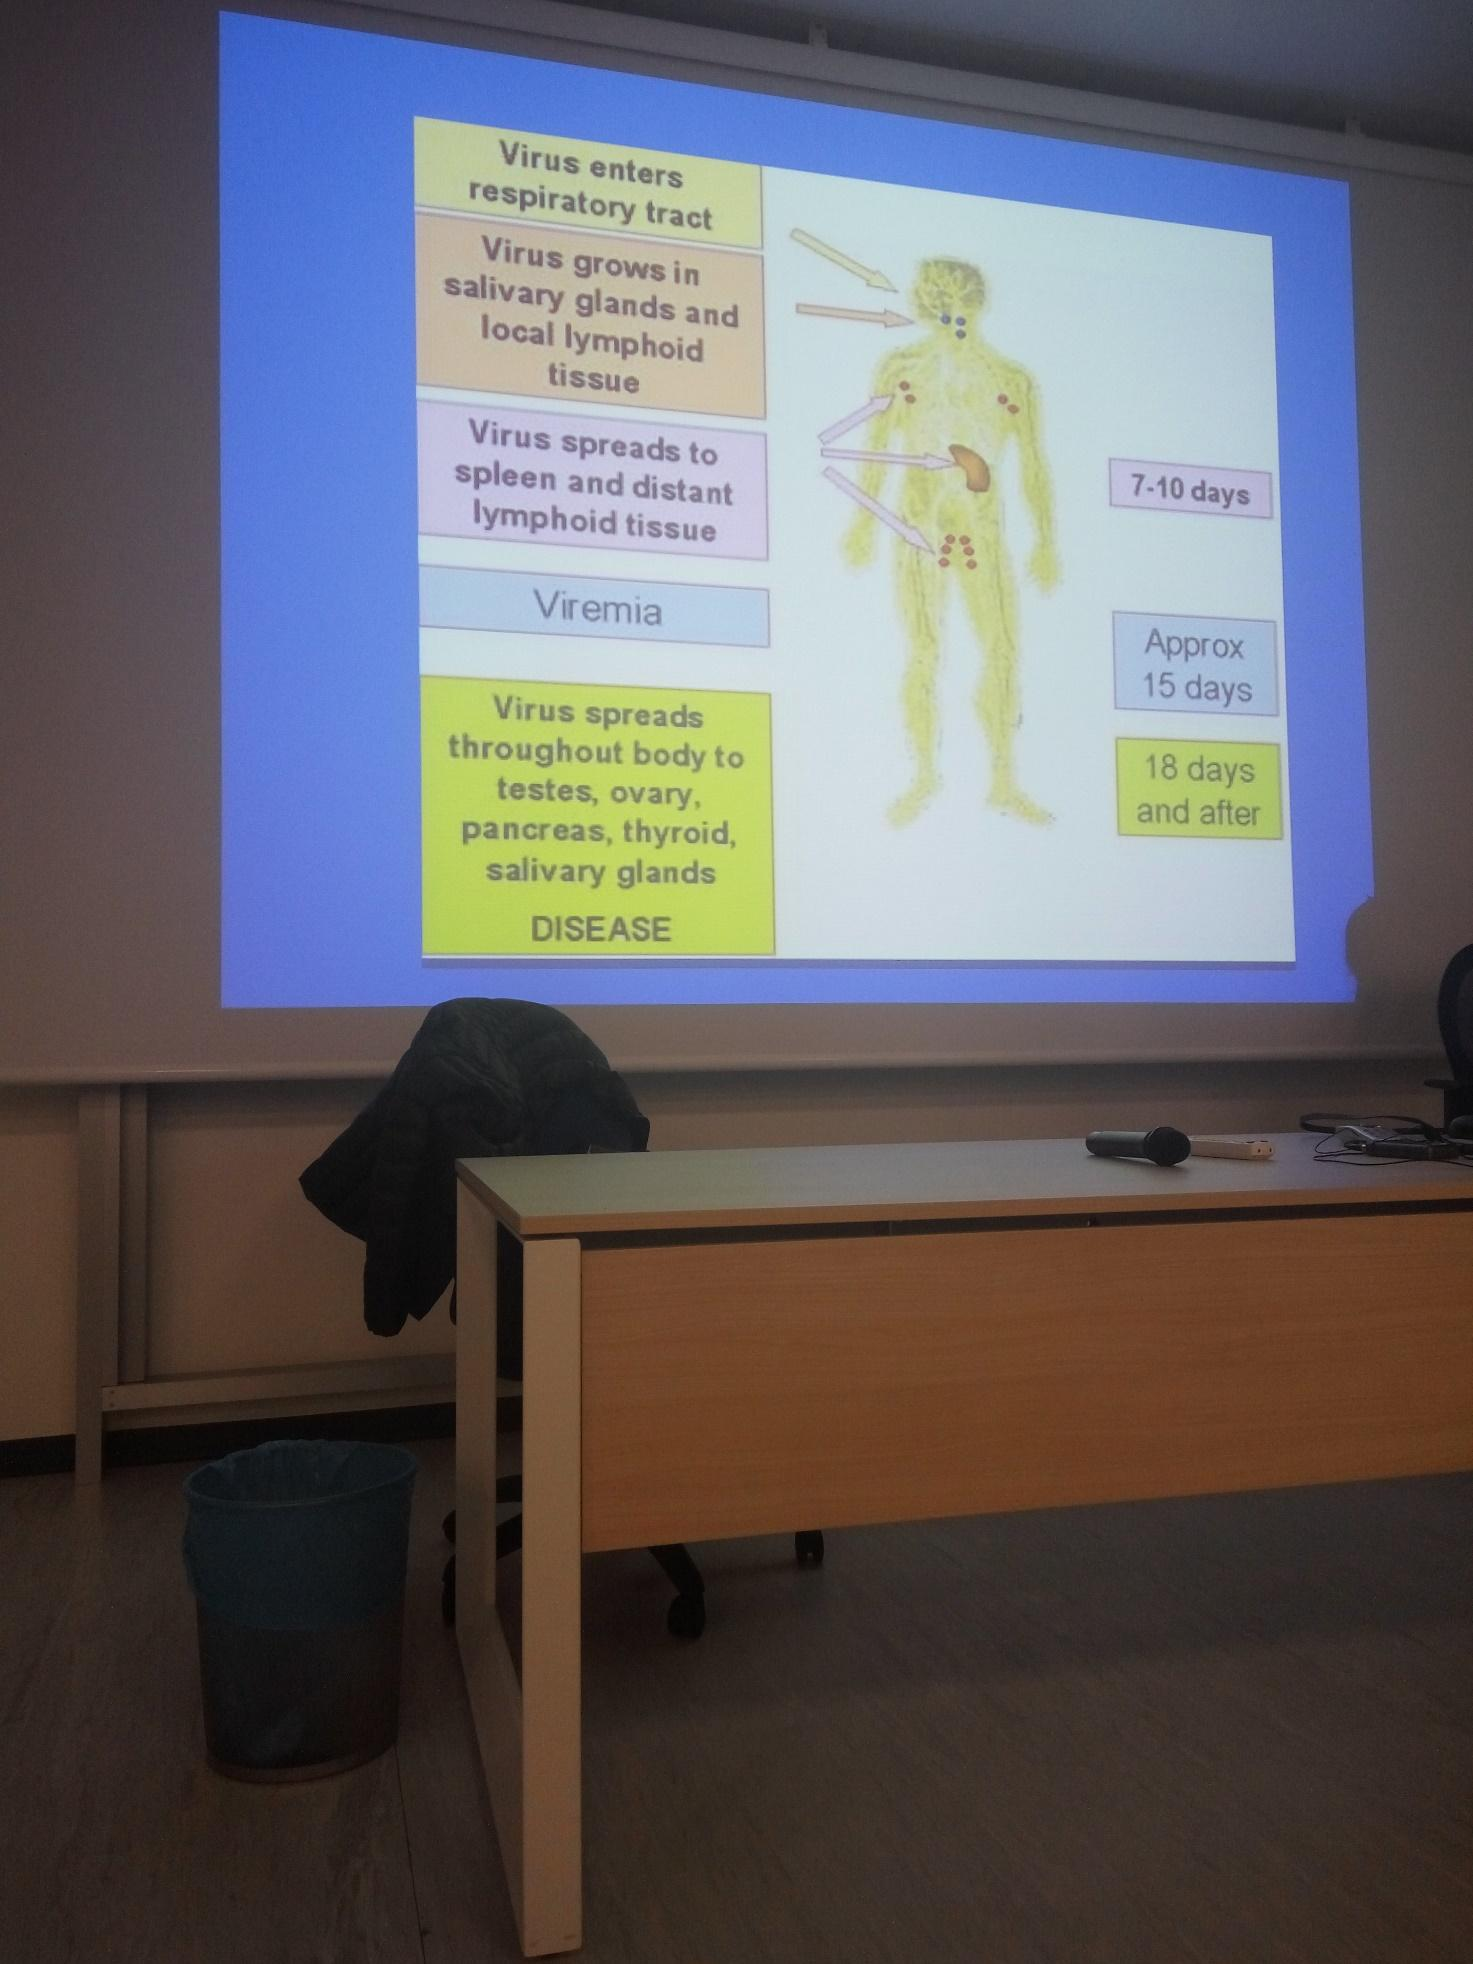
\includegraphics[width=0.8\textwidth]{07/image2.jpeg}
	\end{figure}

Sono
presenti 2 glicoproteine di superficie responsabili dell'adsorbimento e
fusione alla membrana della cellula ospite e gli anticorpi verso queste
glicoproteine neutralizzano l'infettività del virus.

\subsection{Patogenesi}

Trasmissione aerea e si replicazione nel naso-faringe e nei linfonodi
regionali.

Periodo di incubazione 12-24 giorni e successivamente c'è una diffusione
viremica che consente arrivo a numerosi tessuti incluse le meningi,
ghiandole salivari, tiroide, pancreas, ovaio e testicolo.

\subsection{Definizione di caso}

Infiammazione acuta mono o bilaterale delle parotidi o delle ghiandole
salivari da almeno 2 giorni senza altre cause apparenti.

Incubazione 12-24 giorni (media 14-18).

Infezione asintomatica nel 20\% dei casi;

nel 40-50\% può presentarsi in forma aspecifica e nel 30-40\% dei casi
come parotite mono o bilaterale. Risoluzione in modo benigno in 7-10
giorni (soprattutto nel bambino piccolo).

\subsection{Localizzazioni extrasalivari}

Tropismo del virus per tessuto nervoso e parenchimi ghiandolari.

Possono comparire in ogni fase della malattia e in concomitanza con
queste si osserva ripresa della febbre o persistenza oltre il normale
periodo.

\subsection{Complicanze}

\begin{itemize}
\item
  Meningite asettica 5-15\%
\item
  Orchite 25\% età postpuberale (che può portare alla sterilità)
\item
  Ovarite 5\% età post puberale
\item
  Pancreatite 2-5\%
\item
  Sordità (1\textsuperscript{a} causa di sordità acquisita nel bambino)
  1:20.000
\item
  Mortalità 1-3 milione
\item
  Incremento di aborti spontanei in primo trimestre di gravidanza (non
  teratogeno)
\end{itemize}

\subsection{Diagnosi di laboratorio}

Isolamento del virus: saliva, sangue, urine, liquor (anche se non è via
di eliminazione).

Ricerca di anticorpi specifici.

\subsection{Epidemiologia}

È presente in tutto il mondo

In America in età pre-vaccinale erano stimati oltre 200.000 casi/anno,
mentre sono scesi a 3000 casi/anno in epoca post-vaccinale e ora si
attestano a circa 352 casi/anno.

La situazione è simile anche se con numeri diversi in tutti i paesi
industrializzati.

In Europa nel 2011 c'è stata un'epidemia in Bosnia di circa 5000 casi di
cui 41\% complicati.

Andamento nel tempo: endemo-epidemica (3-4 anni).

\begin{figure}[!ht]
\centering
	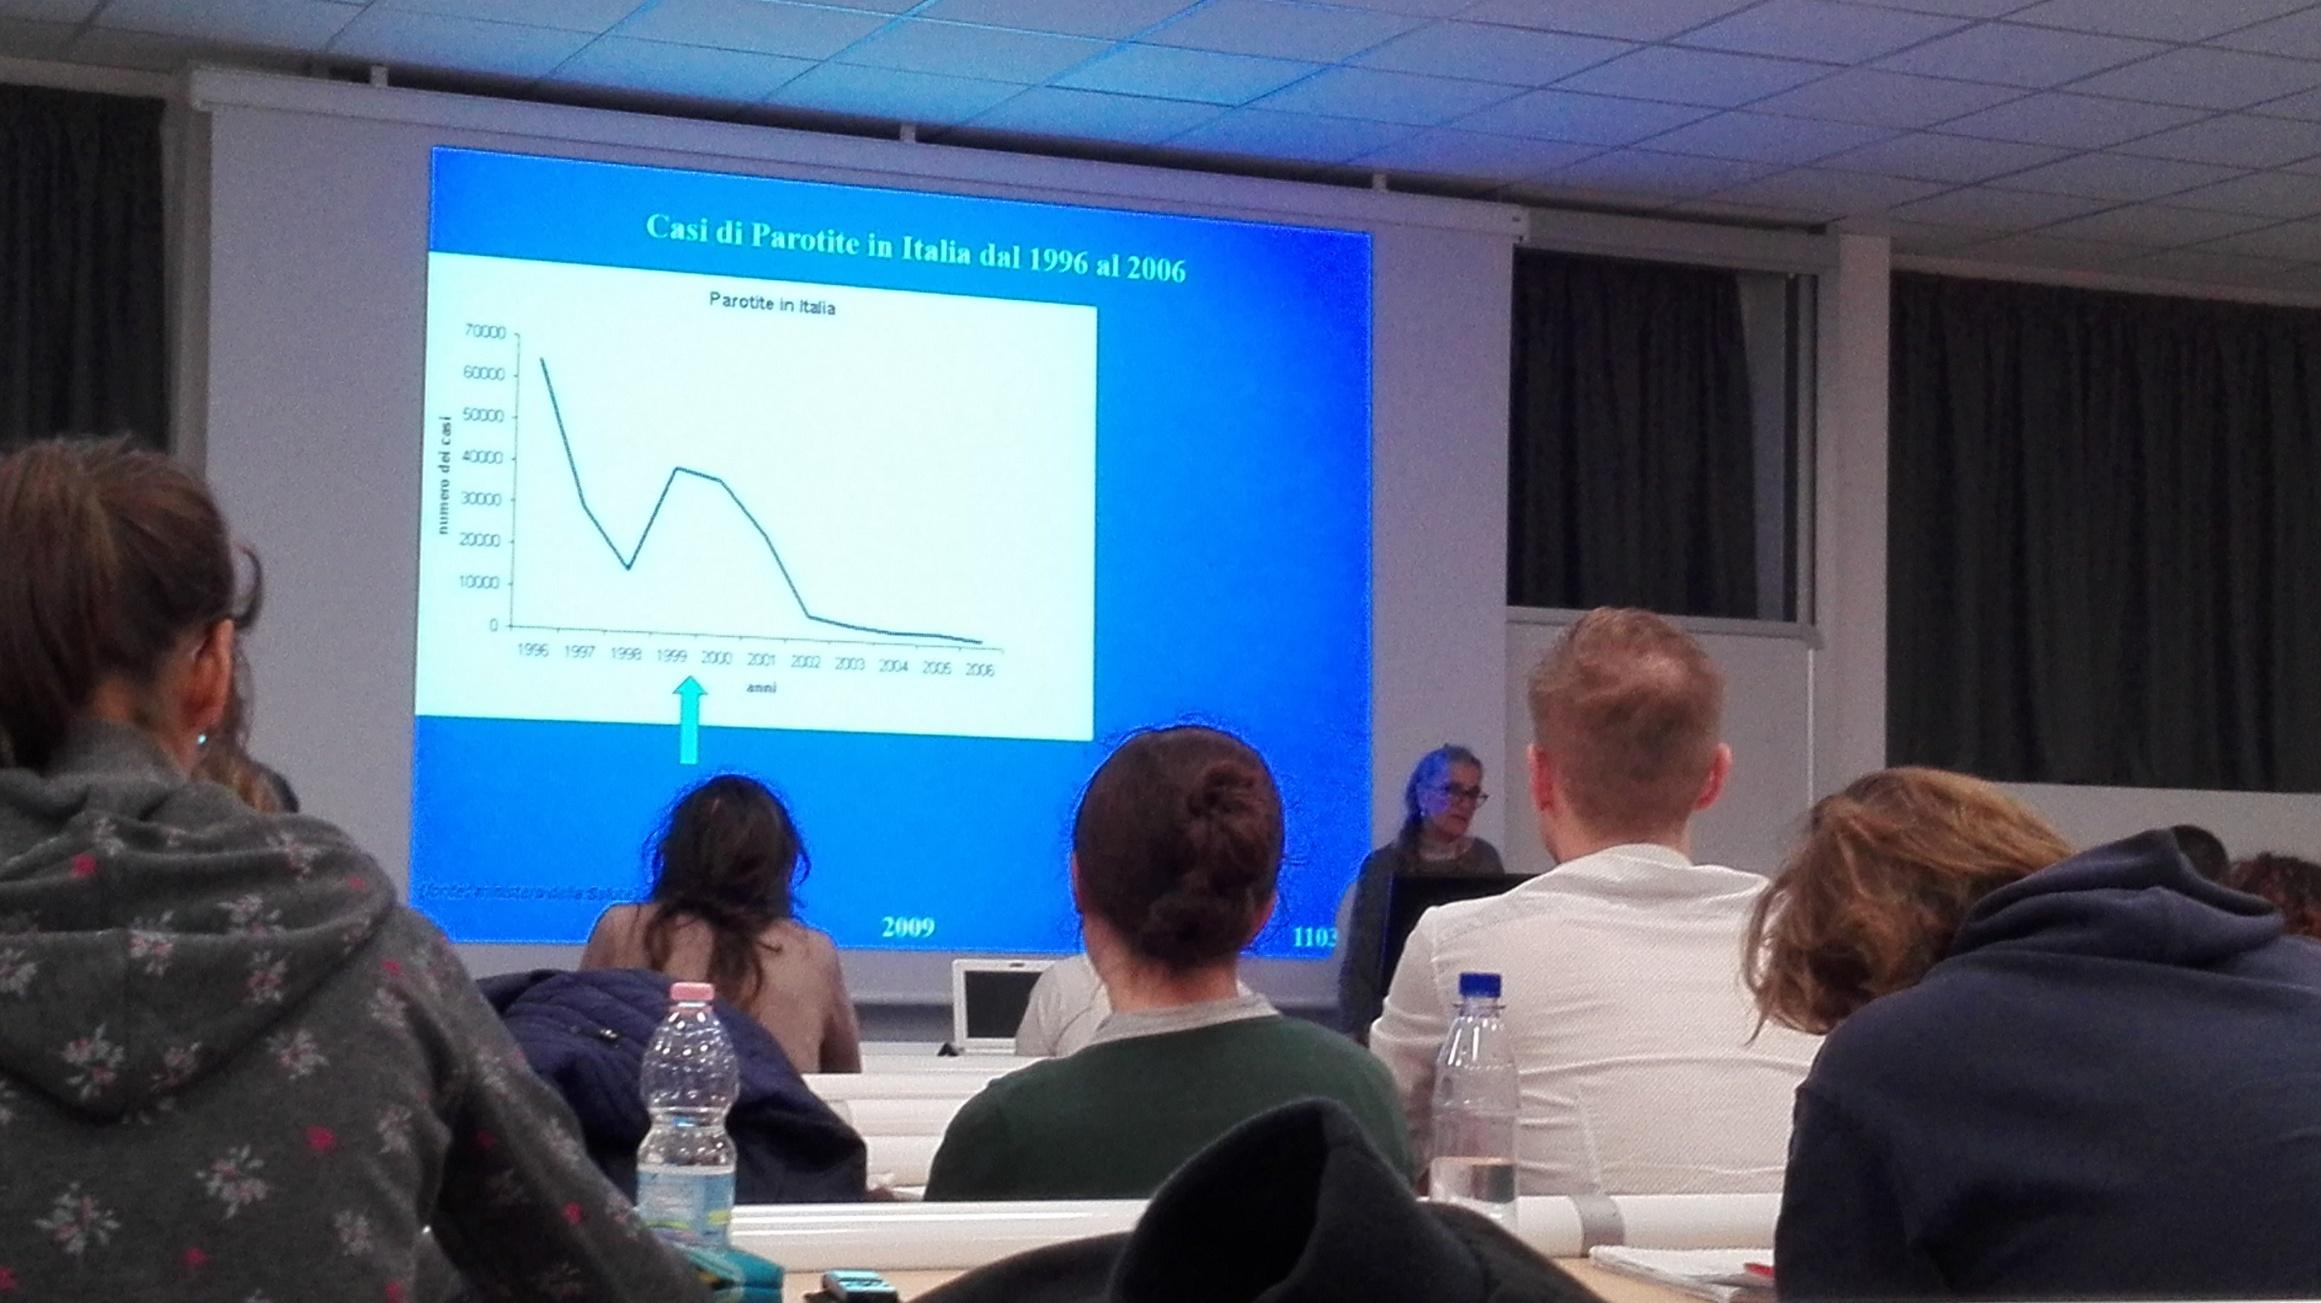
\includegraphics[width=0.8\textwidth]{07/image3.jpeg}
	\end{figure}

Stagionalità:
fine inverno inizio primavera.

Età in epoca pre vaccinale 90\% casi <15 anni, mentre in epoca
post vaccinale 50-80\% dei casi 5-19 anni (complicanze più gravi).

È virus specie-specifico per cui le sorgenti di infezione sono: uomo
malato, portatore precoce e portatore sano.

In Italia a partire dagli anni '90 i casi si sono molto ridotti, ma non
sono ancora arrivati a zero. (`96 oltre 60000 casi, `99 oltre 40000,
2009 circa 1000 casi)

Periodo di contagiosità: da 7 giorni prima e 9 giorni dopo la comparsa
di tumefazione parotidea.

Modalità di trasmissione aerea semidiretta o diretta mediante goccioline
di fludge, saliva.

Immunità persistente.

\subsection{Prevenzione}

\begin{itemize}
\item
  Denuncia obbligatoria notifica di classe 2.
\item
  Isolamento respiratorio per 9 giorni dall'inizio della malattia (se
  non è complicata è isolamento domiciliare).
\item
  Disinfezione e igienizzazione dell'ambiente.
\item
  Inchiesta epidemiologica indagine sui contatti e sulla fonte di
  infezione.
\item
  Vaccinazione: vaccino trivalente MMR (il vaccino per la parotite è
  sempre un vaccino vivo attenuato coltivato in uova embrionate di
  pollo)
\end{itemize}

\subsection{Controindicazioni e precauzioni al vaccino}

\begin{itemize}
\item
  Reazioni allergiche alle proteine dell'uovo
\item
  Gravidanza
\item
  Immunodepressione
\item
  Malattia acuta in atto
\item
  Recente somministrazione di IgG
\end{itemize}


\section{Virus Varicella Zoster}

Malattia virale altamente contagiosa.

Herpes virus a DNA che fa parte degli herpesvirus insieme a HSV1 e HSV2.

Come tutti gli Herpes virus ha la possibilità di mantenersi
nell'organismo.

L'infezione primaria dà luogo alla Varicella. Le reinfezioni possono dar
luogo allo Zoster.

Il virus sopravvive per breve tempo nell'ambiente.

È una malattia dell'infanzia generalmente benigna, ma può avere un
decorso più aggressivo in particolari condizioni: come quando colpisce
adolescenti e adulti, immunocompromessi e quando c'è infezione della
lesione varicellosa da parte dello Streptococcus beta emolitico di tipo
invasivo (fascite necrotizzante) e in bambini in trattamento con acido
acetilsalicilico (perché predispone allo sviluppo della sindrome di
Reye)

\begin{figure}[!ht]
\centering
	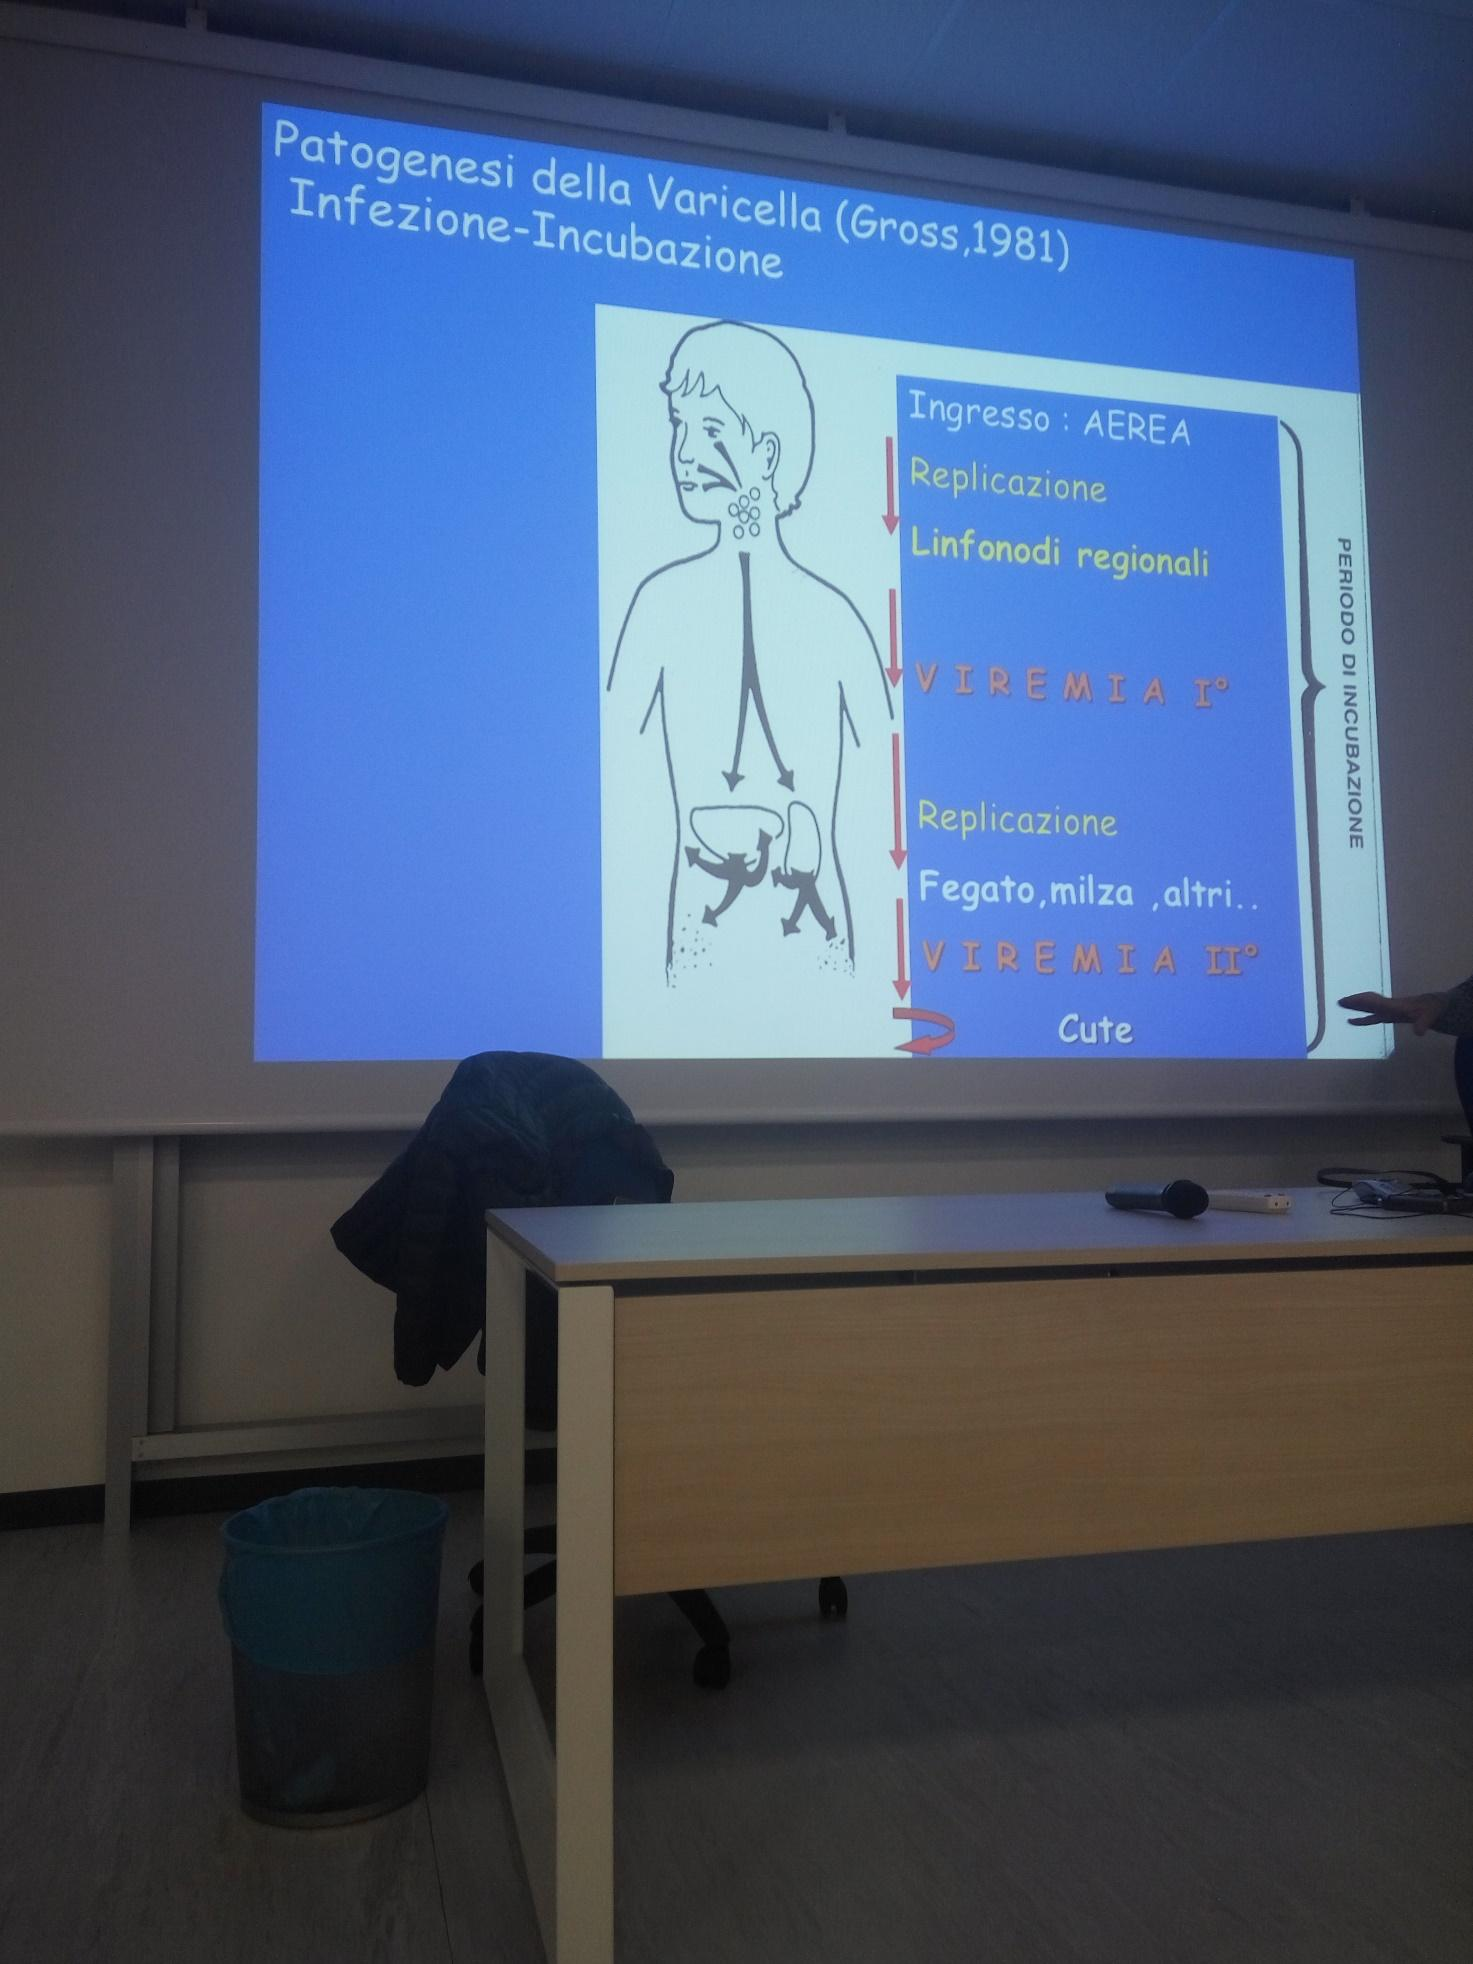
\includegraphics[width=0.8\textwidth]{07/image4.jpeg}
	\end{figure}

\emph{(Wikipedia
Sindrome di Reye: malattia acuta, dall'esito potenzialmente letale, che
colpisce quasi esclusivamente i bambini. È caratterizzata da
manifestazioni patologiche che riguardano prevalentemente il cervello e
il fegato, con encefalopatia acuta e steatosi epatica, che insorgono
rapidamente nel corso di un'infezione virale, spesso dopo l'assunzione
di farmaci a base di acido acetilsalicilico).}

\subsection{Cenni clinici}

Incubazione di 10-21 giorni

Ha 2 fasi viremiche: 1\textsuperscript{o} diffusione agli organi e attiva replicazione
(fegato, milza) e la 2\textsuperscript{o} diffusione alla cute.

Esantema pruriginoso, tipicamente al viso e al tronco, ad ondate
successive.

Le papule evolvono in vescicole poi in pustole quindi in croste.

Si calcolano mediamente circa 300 lesioni (da poche a
>1000).

In giovani adulti spesso più lesioni e più frequenti e più gravi le
complicanze.

Durante l'esantema, VZV può infettare le terminazioni nervose cutanee
stabilendo una infezione latente nei gangli delle radici nervose spinali
che persiste per decenni (probabilmente per tutta la vita).

Nel 15-20\% dei casi si risveglia dopo decenni (in genere dopo 50 anni)
dando luogo allo Zoster (fuoco di Sant'Antonio). Non sempre lo Zoster è
legato a una riattivazione del VZV.

Complicanze rare nei bambini sani. Decorso più aggressivo nel giovane e
adulto.

\subsection{Gruppi a rischio aumentato di VZV}

\begin{itemize}
\item
  Immunodepressi
\item
  Adulti sani
\item
  Neonati da madri con rash da 5 giorni prima a 48 ore dopo il parto.
\end{itemize}

\subsection{Complicanze}

\begin{itemize}
\item
  Infezione batterica delle lesioni
\item
  Manifestazioni a carico del SNC (atassia cerebellare 1/40.000,
  encefalite 1/100.000)
\item
  Polmonite (rara in età infantile)
\item
  Epatite subclinica, linfopenia
\item
  Ospedalizzazione circa 3/1000 casi (dati americani)  
\item
  Mortalità circa 1/60.000 casi (dati americani)
\end{itemize}

\subsection{Accertamento diagnostico}

\begin{itemize}
\item
  Isolamento del virus della varicella da campioni clinici
\item
  Tecniche biomolecolari
\item
  Ricerca degli anticorpi
\end{itemize}

L'infezione conferisce immunità permanente in soggetti immunocompetenti.
Raramente una persona può sviluppare 2 volte la malattia.

\subsection{Epidemiologia}

Specie specifica. Sorgente di infezione è l'uomo che può essere malato o
portatore precoce.

Età 5-10 anni (vaccino è disponibile da poco e perciò non c'è
slittamento dell'età).

Trasmissione: aerea (diretta o semidiretta), per contatto con le lesioni
(personale sanitario a rischio) o verticale transplacentare (come
rosolia può dare problemi al feto).

Contagiosità da 1-2 giorni prima a 4-5 giorni dopo la comparsa del rash.

Eliminazione è molto più lunga negli immunodepressi.

Stagionalità: inverno-inizio primavera.

\subsection{Epidemiologia}

In Italia l'andamento non è modificato presentandosi con plateau
consistente: 100000casi/ anno.

\emph{Gruppi ad alto rischio}:

\begin{itemize}
\item
  immunodepressi
\item
  bambini HIV+ (10\% di incidenza se i bambini si infettano con
  Varicella quando i CD4 sono ridotti del 15\%).
\end{itemize}

Sono dimostrate forme sub cliniche in pazienti trapiantati (midollo
osseo) con dimostrazione di viremia mediante PCR e riattivazione senza
eruzione cutanea ma con dolore.

\emph{Neonati da madre infetta} presentano varicella grave disseminata
nel bambino se l'infezione avviene nei giorni attorno al parto (5 prima-
2 dopo).

\emph{Forma congenita} se contratta tra l'ottava e la
20\textsuperscript{a} settimana; sindrome da varicella congenita
caratterizzata da: difetti a carico del SNC, cute, occhi, arti; basso
peso alla nascita.

Rischio stimato: 2\% dei nati da donne infettate in questo periodo.

\subsection{Profilassi}

\begin{itemize}
\item
  Denuncia obbligatoria classe2
\item
  Isolamento (ospedaliero solo per forme complicate)
\item
  Disinfezione e igienizzazione degli ambienti
\item
  Immunoprofilassi Passiva IgG specifiche (anche preparato per endovena)
\item
  Vaccino vivo ed attenuato
\end{itemize}

\subsection{Vaccino}

\begin{itemize}
\item
  Composizione: virus attenuato (ceppo Oka)
\item
  Efficacia 95\% (range, 95\%-100\%)
\item
  Durata immunità \textgreater{}7 anni
\item
  Schedula 1 dose (\textless{}13 anni)
\item
  Può essere somministrato simultaneamente al trivalente ma in zone
  diverse (MMR VZ) oppure come tetravalente (MMRVZ)
\end{itemize}

È prevista la vaccinazione per:

\begin{itemize}
\item
  Bambini sani entro i 2 anni di età
\item
  Bambini ad alto rischio di gravità
\item
  Adulti suscettibili offerta attiva adolescenti e giovani (11-18 anni)
\item
  Adulti a rischio per attività professionale e soggetti con patologie
  quali: IRC, malattie linfoproliferative, candidati a trapianto
  epatico, renale, midollare
\end{itemize}

Avvertenze particolari in applicazione del vaccino in bambini leucemici:
remissione da almeno 2 mesi, sospensione della chemioterapia da 1
settimana prima a 1 settimana dopo la vaccinazione e con trasformazione
blastica normale.

\subsection{PNPV 2016-2018}

Raggiungimento e mantenimento di copertura vaccinali per 1 dose di
vaccinazione antivaricella che deve raggiungere almeno il 95\% entro i 2
anni di età a partire dalla coorte 2014

Raggiungimento e mantenimento di coperture vaccinali con 2 dosi di
vaccinazione antivaricella in almeno il 95\% dei bambini di 5-6 anni a
partire dalla coorte 2014.

\subsection{Reazioni avverseì}

\begin{itemize}
\item
  Locali 30\%
\item
  Rash 5\%
\item
  Febbre (\textgreater{}37,5 \textsuperscript{o}C) 10\%
\end{itemize}

\subsection{Controindicazioni alla vaccinazione}

\begin{itemize}
\item
  Malattia acuta con o senza febbre (controindicazione temporanea)
\item
  Ipersensibilità alla neomicina (per tracce all'interno del preparato)
\item
  Leucopenia \textless{}1200 /mm\textsuperscript{3}
\item
  Terapia immunosoppressiva
\item
  Gravidanza (evitare per almeno 3 mesi)
\item
  Somministrazione di immunoglobuline iperimmuni antiVZV nei 3 mesi
  precedenti
\item
  Tubercolosi non trattata
\end{itemize}

\subsection{Profilassi post esposizione con immunoglobuline (VZIG)}

Efficaci nel prevenire o ridurre la gravità della malattia solo se
somministrate entro le 96 ore.

Indicazioni:

\begin{itemize}
\item
  Bambino suscettibile e immunocompromesso
\item
  Donna in gravidanza e suscettibile
\item
  Neonato la cui madre ha presentato la varicella da 5 giorni prima a 48
  ore dopo il parto
\item
  Nato da parto prematuro ricoverato con madre suscettibile
\end{itemize}